% optB: trapezoid outer TL-TR-BR-BL + solid BL-TR + dashed TL-BR
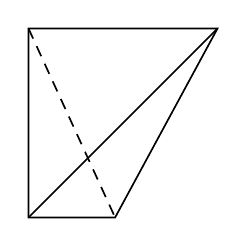
\begin{tikzpicture}[line width=0.6pt]
\coordinate (BL) at (0,0);
\coordinate (BR) at (1.1,0);
\coordinate (TR) at (2.4,2.4);
\coordinate (TL) at (0,2.4);
\draw[draw=black] (BL)--(BR)--(TR)--(TL)--cycle;
\draw[draw=black] (BL)--(TR);
\draw[draw=black,dash pattern=on 4pt off 3pt] (TL)--(BR);
\end{tikzpicture}
